\subsubsection{Kennzahlen}
Zunächst einmal können die Spannungspegel definiert werden: 
\begin{itemize}
	\item Speisespannung PCB (vom Netzteil): \textbf{24V}
	\item Treiberspeisung Endstufen (PVDD): \textbf{15V}
	\item Digitale Speisung Endstufen (DVDD): \textbf{3.3V}
	\item Speisung Milan-Modul: \textbf{5V}
\end{itemize}
Aus dem Datenblatt des DAEX19QLP-4 \cite{DAEX19QLP4spec} kann die Nominalimpedanz von 4 Ohm bestimmt werden. Da dieser Exciter mit maximal 5 Watt betrieben wird, kann nun die erwartete Effizienz eines Kanals aus Abbildung \ref{pics:tas5720_efficiency_4ohm} abgelesen werden: \textit{ca.} 82.5\%. Dadurch lässt sich auch die benötigte Gesamtleistung (rms und peak) pro Kanal berechnen:
\begin{equation}
	P_{ch(nom)} = \frac{P_{out}}{\mu_{amp} @ 15V} \rightarrow P_{ch(nom)} = \frac{5}{0.825} = \textbf{6.06 W}
	\label{eq:pwr_per_channel_rms}
\end{equation}
\begin{equation}
	P_{ch(peak)} = P_{ch(nom)} \cdot Crest \rightarrow P_{ch(peak)} = 6.06W \cdot 10^{\frac{6}{10}} = \textbf{24.24 W}
	\label{eq:pwr_per_channel_peak}
\end{equation}
Somit beträgt die benötigte Gesamtleistung und die empfohlene Nominalleistung der Speisung bei Volllast:
\begin{equation}
	P_{max} = N_{Exciter} \cdot P_{ch} \rightarrow P_{max} = 6 \cdot 6.1 W = \textbf{36.6 W}
\end{equation}
\begin{equation}
	P_{supply(nom.)} = P_{max} \cdot 2 \rightarrow P_{supply(nom.)} = 36.6W \cdot 2 = \textbf{73.2 W} (@ 15V)
\end{equation}
\begin{figure}[H]
	\centering
	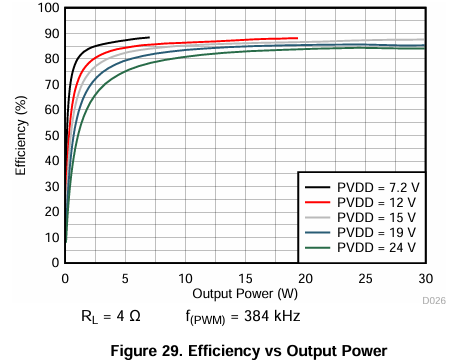
\includegraphics[width = \textwidth*1/2]{pictures/tas5720l_efficiency_4Ohms.png}
	\caption{Effizienz des TAS5720 bei 4 Ohm}
	\label{pics:tas5720_efficiency_4ohm}
\end{figure}
\subsubsection{Speisungsaufbau}
Nun können verschiedene Ansätze gewählt werden um die Speisung zu realisieren:
\begin{itemize}
	\item Ein einzelner IC regelt die Spannung für alle sechs Endstufen.
	\item Zwei ICs speisen jeweils drei Endstufen.
	\item Drei ICs speisen jeweils zwei Endstufen.
	\item Jeder IC hat eine eigene Spannungsregelung.
\end{itemize}
Zudem muss entschieden werden, ob Linearregler oder Schaltregler, oder eine Kombination aus beiden verwendet werden müssen\footnote{Siehe auch \cite{switchingreg_linreg}}. Hierzu könnte auch eine Zwischenspannung von beispielsweise 17V nötig sein, um die Verlustleistung der LDOs zu begrenzen.
\begin{itemize}
	\item[] \textbf{\large Schaltregler}
	\begin{itemize}
		\item Vorteile
		\begin{itemize}
			\item [\bullet]Effizient, wenig Verlustleistung
			\item [\bullet]Leistungen können (fast) direkt umgerechnet werden
			\item [\bullet]Grosse Zahl an Varianten erhältlich
			\item [\bullet]Leistungsstark
		\end{itemize}
		\item Nachteile
		\begin{itemize}
			\item [\bullet]Durch Schaltvorgang Ripple- und Noise auf der Speisung
			\item [\bullet]Komplex im Aufbau
			\item [\bullet]Bauteile müssen sorgfältig ausgewählt werden.
		\end{itemize}
	\end{itemize}
	\item[] \textbf{\large Linearregler}
	\begin{itemize}
		\item Vorteile
		\begin{itemize}
			\item [\bullet]Einfach im Aufbau
			\item [\bullet]Wenig Bautteile nötig
			\item [\bullet]Günstig
			\item [\bullet]Varianten mit extrem wenig Noise erhältlich.
		\end{itemize}
		\item Nachteile
		\begin{itemize}
			\item [\bullet]Rein \textquotedbl{}kontrollierter Spannungsabfall\textquotedbl{}. Der Laststrom wird 1:1 aus der Hauptspannung bezogen!
			\item [\bullet]Durch Verlustleistung nur bis begrenzte Lastströme möglich
		\end{itemize}
	\end{itemize}
\end{itemize}
Aus der Gleichung \ref{eq:pwr_per_channel_rms} der maximale Effektiv- und Spitzenstrom berechnet werden, wobei hier ein Crest-Factor von 6dB verwendet wird.
\begin{equation}
	I_{ch(rms)} = \frac{P_{ch(max)}}{U_{supply}} \rightarrow I_{ch(max,rms)} = \frac{6.06W}{15V} = \textbf{0.404 A}
	\label{eq:rms_current_per_channel}
\end{equation}
\begin{equation}
	I_{ch(peak)} = \frac{P_{ch(max)} \cdot Crest}{U_{supply}}  \rightarrow I_{ch(max,rms)} = \frac{6.06W \cdot 10^{\frac{6}{10}}}{15V} = \textbf{1.608 A}
	\label{eq:peak_current_per_channel}
\end{equation}
Hinzu kommt die Stromaufnahme des Milan-Moduls, welches mit 5V betrieben wird und je nach konfiguration \textit{ca.} 350 bis 500mA beträgt\footnote{Dies wurde per E-Mail mitgeteilt und ist in keinem Datenblatt ausgegeben.}.
\begin{equation}
	I_{Module} = \textbf{350 - 500mA @ 5V}
\end{equation}
\paragraph{Speisung mit nur Linearreglern} Die Verwendung von ausschliesslich Linearreglern hätte zwar einige Vorteile im Rauschverhalten, jedoch würde der in Gleichung \ref{eq:peak_current_per_channel} berechnete Spitzenstrom \textit{pro Kanal} aus der Hauptspeisung bezogen werden. Dies ergäbe, allein für die Endstufen und mit angenommen 100\% Effizienz, bei einem 24V-Netzteil eine Leistungsanforderung von mindestens $P_{peak} = I_{peak} \cdot N_{ch} \cdot U_{supply} \rightarrow P_{peak} = 1.608A \cdot 6 \cdot 24V = \textbf{231.5W}$ benötigt wird. Zwar gibt es Netzteile mit solchen Leistungen, jedoch wären die Kosten und Gewicht sehr hoch für diese Anwendung.
\subsection{Simulation der Last und passiven Entkopplung}
Um das Lastverhalten so detailliert wie möglich zu simulieren, muss ein Signalverlauf erzeugt werden, dessen Spitzenwert und Crestfaktor der letztendlichen Anwendung so nahe wie möglich kommt. Zu diesem Zweck wurde von der Webseite der AES ein Lautsprecher-Testsignal heruntergeladen \footnote{Siehe: \cite{aes75}}. Dieses Signal ist ein auf Musikinhalte zugeschnittener Pinkes Rauschen (Dateiname: \textit{Music-Noise\_48kHz}). Mittels dem Open Source Programm Audacity wurde das Signal ein einer Stelle mit einer hohen Spitze als einzelne Samplewerte exportiert. Diese Werte konnten dann in das Simulationsprogramm NI Multisim als PWL-Spannungsquelle (\textit{PIECEWISE\_LINEAR\_VOLTAGE}) importiert werden. Mittels eines Skalierungs-Bausteins (\textit{VOLTAGE\_CONTROLLED\_PIECEWISE\_LINEAR\_SOURCE}) kann dieses Signal umgewandelt werden, sodass schliesslich eine Last gesteuert werden kann (\textit{VOLTAGE\_CONTROLLED\_RESISTOR\_VIRTUAL}). 
\paragraph{Keine Simulationsmodelle des TAS5720}Sowohl auf der Webseite von Texas Instruments als auch in PSpice\footnote{Die Simulationssoftware von Texas Instruments} waren zum Zeitpunkt der Arbeit keine Simulationsmodelle des TAS5720 verfügbar. Daher konnte nur aus der Effizienz und der bekannten Last das Verhalten des TAS5720 ermittelt werden: Die Skalierung des Simulations-Bausteins wurde so angepasst, dass die simulierte Leistungsspitze über dem Lastwiderstand genau den berechneten Spitzenwert aus Gleichung \ref{eq:pwr_per_channel_peak} erreichte. Es konnten dabei auch zwei oder mehr Lasten parallel betrieben werden, was einem Parallelbetrieb von mehreren Kanälen entspricht. Abbildung \ref{pic:simulation_load} zeigt dem Simulationsaufbau und Abbildung \ref{plot:load_transient} die damit erzeugte Transiente.
Danach wurde mit einer idealen 15V-Spannungsquelle und einem 250mOhm\footnote{Was einer eher schlechten Speisung entspricht.} Innenwiderstand die Speisung simuliert. Die somit entstehende Stromspitze erzeugte nun einen entsprechenden Speisungsabfall (Abbildung \ref{plot:load_transient_nofilter}).
\begin{figure}[H]
	\centering
	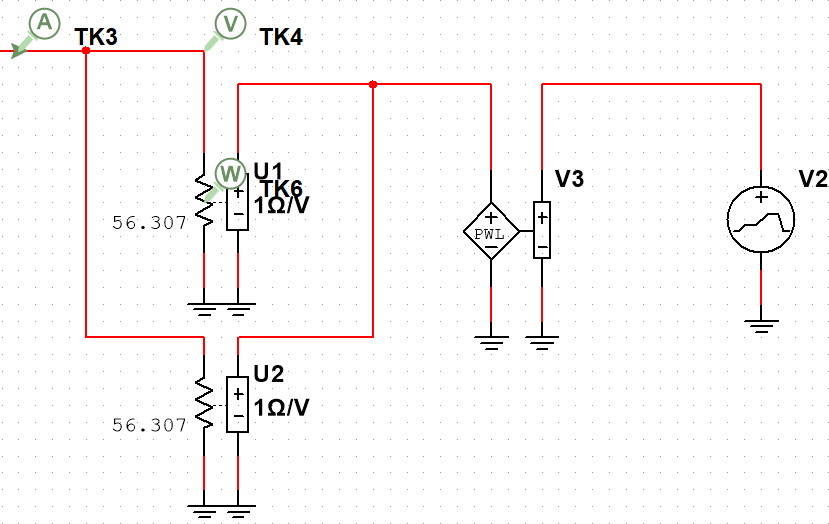
\includegraphics[width=\textwidth*6/8]{pictures/simu_load.png}
	\caption{Aufbau der Lastsimulation}
	\label{pic:simulation_load}
\end{figure}
\begin{figure}[H]
	\centering
	\begin{tikzpicture}
		\pgfplotsset{minor grid style={dashed}}
		\begin{axis}[
			width = \linewidth*3/4,
			height = \linewidth*3/8,
			xlabel = {Zeit in [s]},
			ylabel = {Leistung in [W]},
			xmin=0, xmax=0.01,
			ymin=0, ymax=25,
			grid=both,
			ymajorgrids=true,
			yminorgrids=true,
			xmajorgrids=true,
			yminorticks=true,
			minor y tick num=4
			]
			\addplot [
				red
				] table [
				x=X, 
				y=Y, 
				col sep=comma
				] {data/Load_simulation.csv};
		\end{axis}
	\end{tikzpicture}
	\caption{Leistungstransiente einer Last}
	\label{plot:load_transient}
\end{figure}
\begin{figure}[H]
	\centering
	\begin{tikzpicture}
		\pgfplotsset{set layers}
		\pgfplotsset{minor grid style={dashed}}
		\begin{axis}[
			scale only axis,
			width = \linewidth*3/4,
			height = \linewidth*3/8,
			axis y line=left,
			xlabel = {Zeit in [s]},
			ylabel = {\ref{plot:U_drop}Spannung in [V]},
			ylabel style = {align=center},
			xmin=0, xmax=0.01,
			ymin=12, ymax=15,
			grid=both,
			minor y tick num=1
			]
			\addplot [
			blue
			] table [
			x=X, 
			y=U, 
			col sep=comma
			] {data/Load_Transient_nofilter.csv};\label{plot:U_drop}
		\end{axis}
		\begin{axis}[
			scale only axis,
			width = \linewidth*3/4,
			height = \linewidth*3/8,
			axis y line=right,
			axis x line=none,
			ylabel = {\ref{plot:I_transient} Strom in [A]},
			ylabel style = {align=center},
			xmin=0, xmax=0.01,
			ymin=0, ymax=6,
			minor y tick num=1
			]
			\addplot [
			red
			] table [
			x=X, 
			y=I, 
			col sep=comma
			] {data/Load_Transient_nofilter.csv}; \label{plot:I_transient}
		\end{axis}
	\end{tikzpicture}
	\caption{Strom und Spannung bei einer Leistungstransiente (zwei Lasten parallel)}
	\label{plot:load_transient_nofilter}
\end{figure}
Der Spannungseinbruch und die Stromspitze mussten nun möglichst reduziert werden. Insbesondere die Stromspitze würde bei sechs Kanälen zu einem Spitzenstrom vom 9 A führen.
\subsubsection{Parameter-Sweep}
Es wurde nun eine Induktion in Serie und eine Kapazität in parallel zur Last eingefügt. Die Induktion wurde mit einem ESR von 120mOhm und die Kapazität mit ESR von 25mOhm simuliert. Abbildung \ref{pic:simulation_complete} zeigt den kompletten Simulationsaufbau. Mit einem Parameter-Sweep können nun die optimalen Bauteilwerte eruiert werden (\textit{So viel wie nötig, so wenig wie möglich}). Da dies jedoch pro Durchgang nur für einen Bauteilwert möglich ist, wurde die Kapazität von 0 F an in 100uF-Schritten erhöht und ein Parameter-Sweep auf die Induktivität durchgeführt. Dabei wurde pro Durchgang der Speisungsstrom und die Lastspannung aufgezeichnet. Der Übersichtlichkeit halber, wurden diese in separate Diagramme aufgezeichnet. Abbildungen \ref{pic:supplycurrent_loadvoltage_0F} bis \ref{pic:supplycurrent_loadvoltage_400uF} zeigen das Verhalten von Lastspannung und Speisungsstrom unter verschiedenen Voraussetzungen.
\begin{figure}[H]
	\centering
	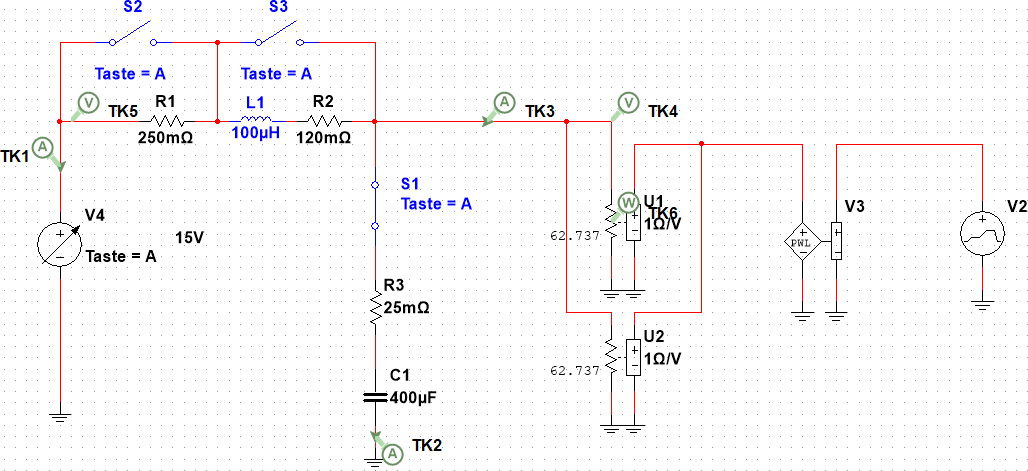
\includegraphics[width=\textwidth*6/8]{pictures/simu_cap_sweep_schematic.png}
	\caption{Kompletter Aufbau der Simulation}
	\label{pic:simulation_complete}
\end{figure}
\begin{figure}[H]
	\centering
	\begin{subfigure}{\textwidth*6/13}
		\centering
		\includegraphics[width=\textwidth]{pictures/2LoadsParallel_Lastspannung bei 0F Kapazität_IndSweep0Hto400uH.pdf}
		\caption{Lastspannung bei 0F und 0-400uH}
		\label{pic:loadvoltage_0F}
	\end{subfigure}
	\hfill
	\begin{subfigure}{\textwidth*6/13}
		\centering
		\includegraphics[width=\textwidth]{pictures/2LoadsParallel_Speisestrom bei 0F Kapazität_IndSweep0Hto400uH.pdf}
		\caption{Speisestrom bei 0F und 0-400uH}
		\label{pic:supplycurrent_0F}
	\end{subfigure}
	\caption{Lastspannung und Speisestrom bei 0F und 0-400uH}
	\label{pic:supplycurrent_loadvoltage_0F}
\end{figure}
\begin{figure}[H]
	\centering
	\begin{subfigure}{\textwidth*6/13}
		\centering
		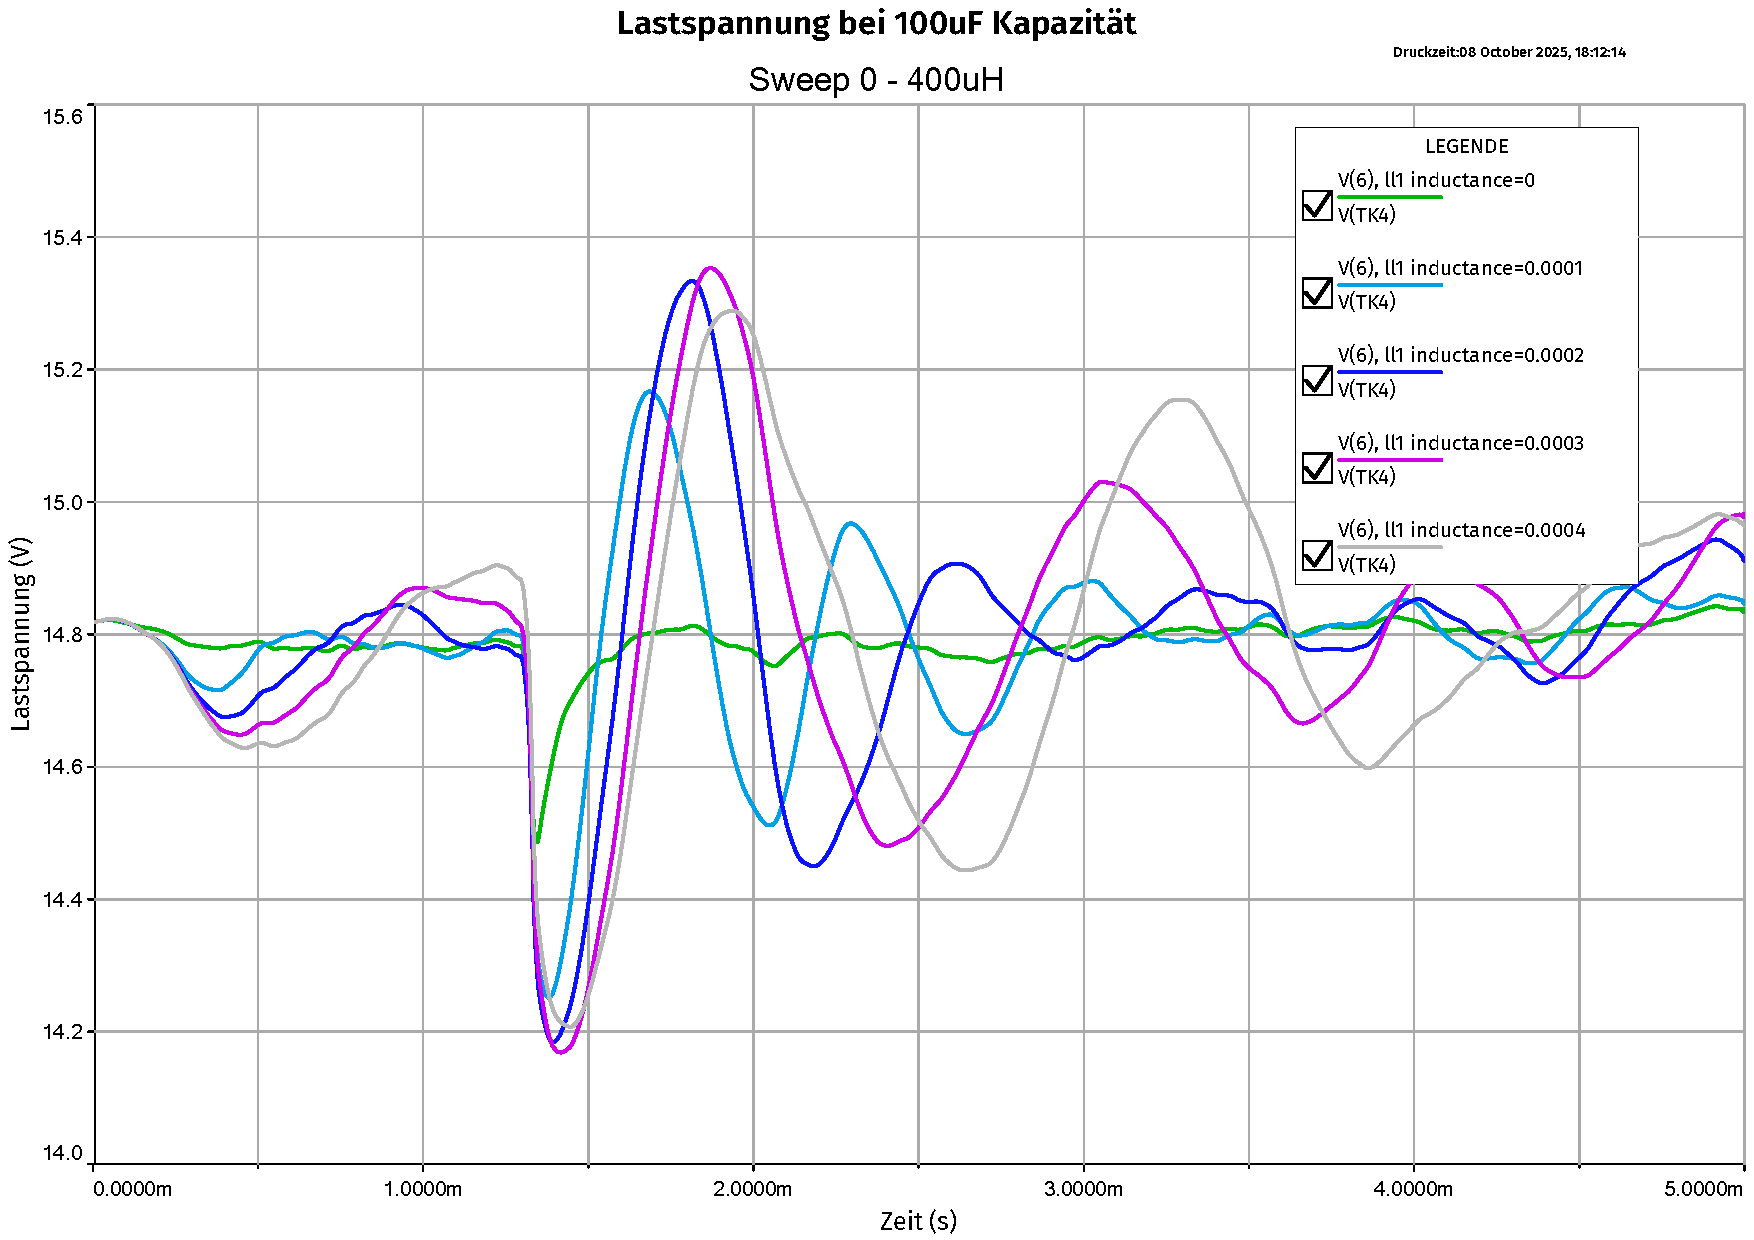
\includegraphics[width=\textwidth]{pictures/2LoadsParallel_Lastspannung bei 100uF_IndSweep0Hto400uH.pdf}
		\caption{Lastspannung bei 100uF und 0-400uH}
		\label{pic:loadvoltage_100uF}
	\end{subfigure}
	\hfill
	\begin{subfigure}{\textwidth*6/13}
		\centering
		\includegraphics[width=\textwidth]{pictures/2LoadsParallel_Speisestrom bei 100uF Kapazität_IndSweep0Hto400uH.pdf}
		\caption{Speisestrom bei 100uF und 0-400uH}
		\label{pic:supplycurrent_100uF}
	\end{subfigure}
	\caption{Lastspannung und Speisestrom bei 100uF und 0-400uH}
	\label{pic:supplycurrent_loadvoltage_100uF}
\end{figure}
\begin{figure}[H]
	\centering
	\begin{subfigure}{\textwidth*6/13}
		\centering
		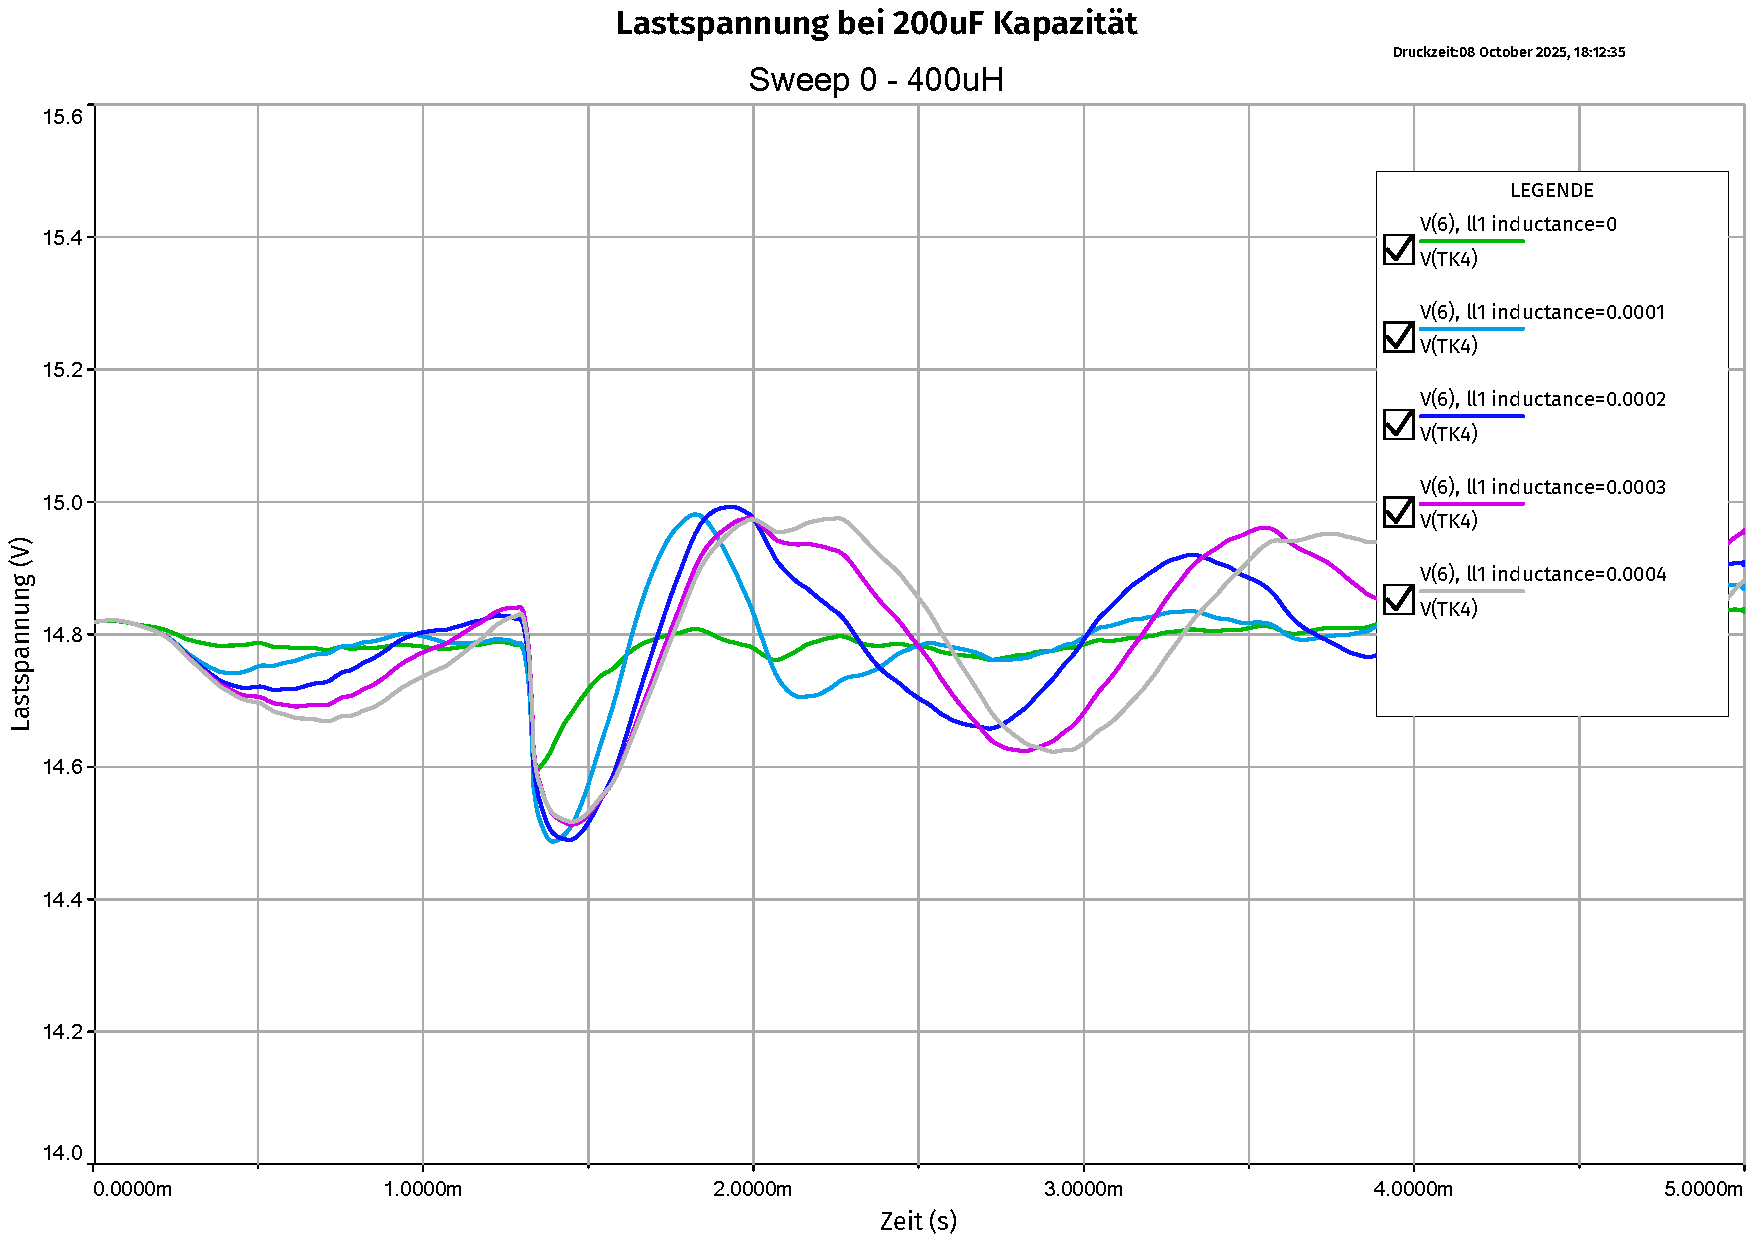
\includegraphics[width=\textwidth]{pictures/2LoadsParallel_Lastspannung bei 200uF_IndSweep0Hto400uH.pdf}
		\caption{Lastspannung bei 200uF und 0-400uH}
		\label{pic:loadvoltage_200uF}
	\end{subfigure}
	\hfill
	\begin{subfigure}{\textwidth*6/13}
		\centering
		\includegraphics[width=\textwidth]{pictures/2LoadsParallel_Speisestrom bei 200uF Kapazität_IndSweep0Hto400uH.pdf}
		\caption{Speisestrom bei 200uF und 0-400uH}
		\label{pic:supplycurrent_200uF}
	\end{subfigure}
	\caption{Lastspannung und Speisestrom bei 200uF und 0-400uH}
	\label{pic:supplycurrent_loadvoltage_200uF}
\end{figure}
\begin{figure}[H]
	\centering
	\begin{subfigure}{\textwidth*6/13}
		\centering
		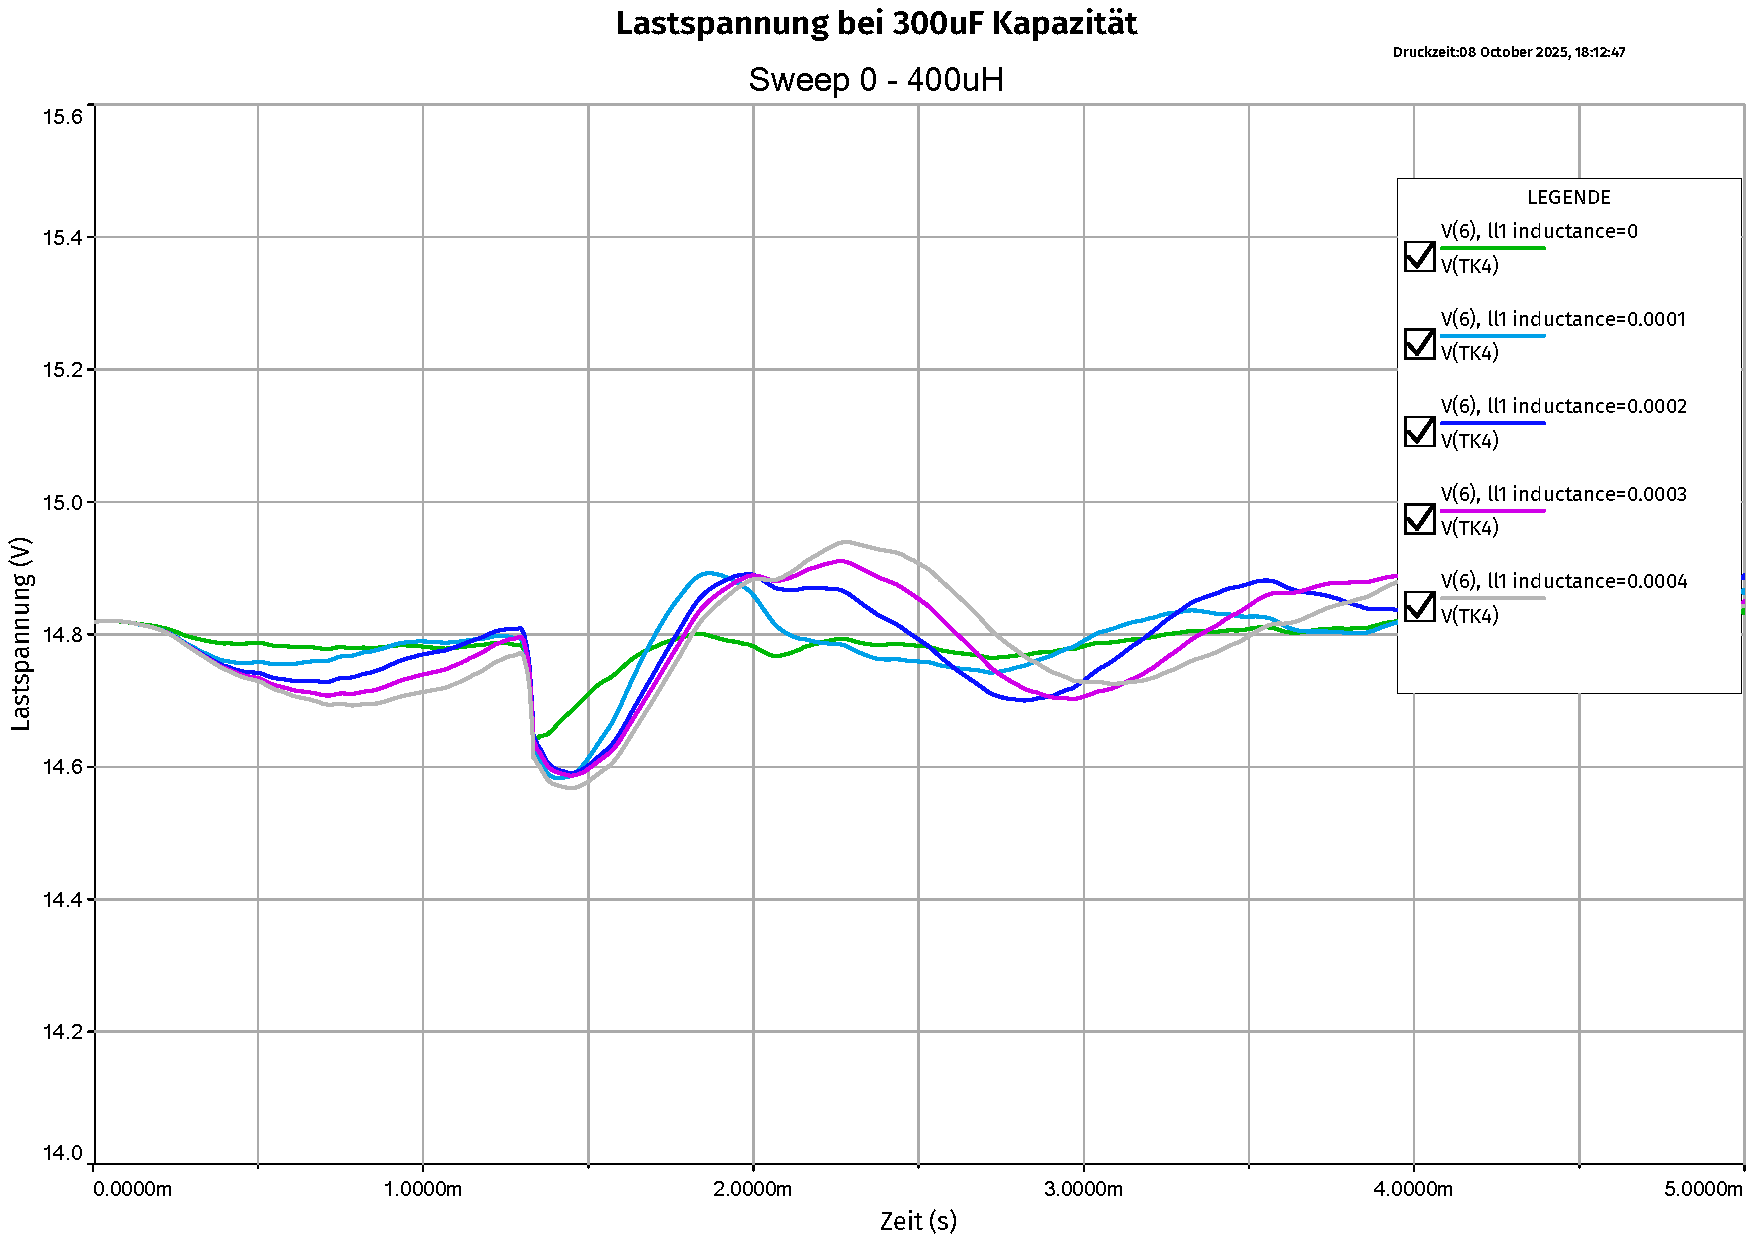
\includegraphics[width=\textwidth]{pictures/2LoadsParallel_Lastspannung bei 300uF_IndSweep0Hto400uH.pdf}
		\caption{Lastspannung bei 300uF und 0-400uH}
		\label{pic:loadvoltage_300uF}
	\end{subfigure}
	\hfill
	\begin{subfigure}{\textwidth*6/13}
		\centering
		\includegraphics[width=\textwidth]{pictures/2LoadsParallel_Speisestrom bei 300uF Kapazität_IndSweep0Hto400uH.pdf}
		\caption{Speisestrom bei 300uF und 0-400uH}
		\label{pic:supplycurrent_300uF}
	\end{subfigure}
	\caption{Lastspannung und Speisestrom bei 300uF und 0-400uH}
	\label{pic:supplycurrent_loadvoltage_300uF}
\end{figure}
\begin{figure}[H]
	\centering
	\begin{subfigure}{\textwidth*6/13}
		\centering
		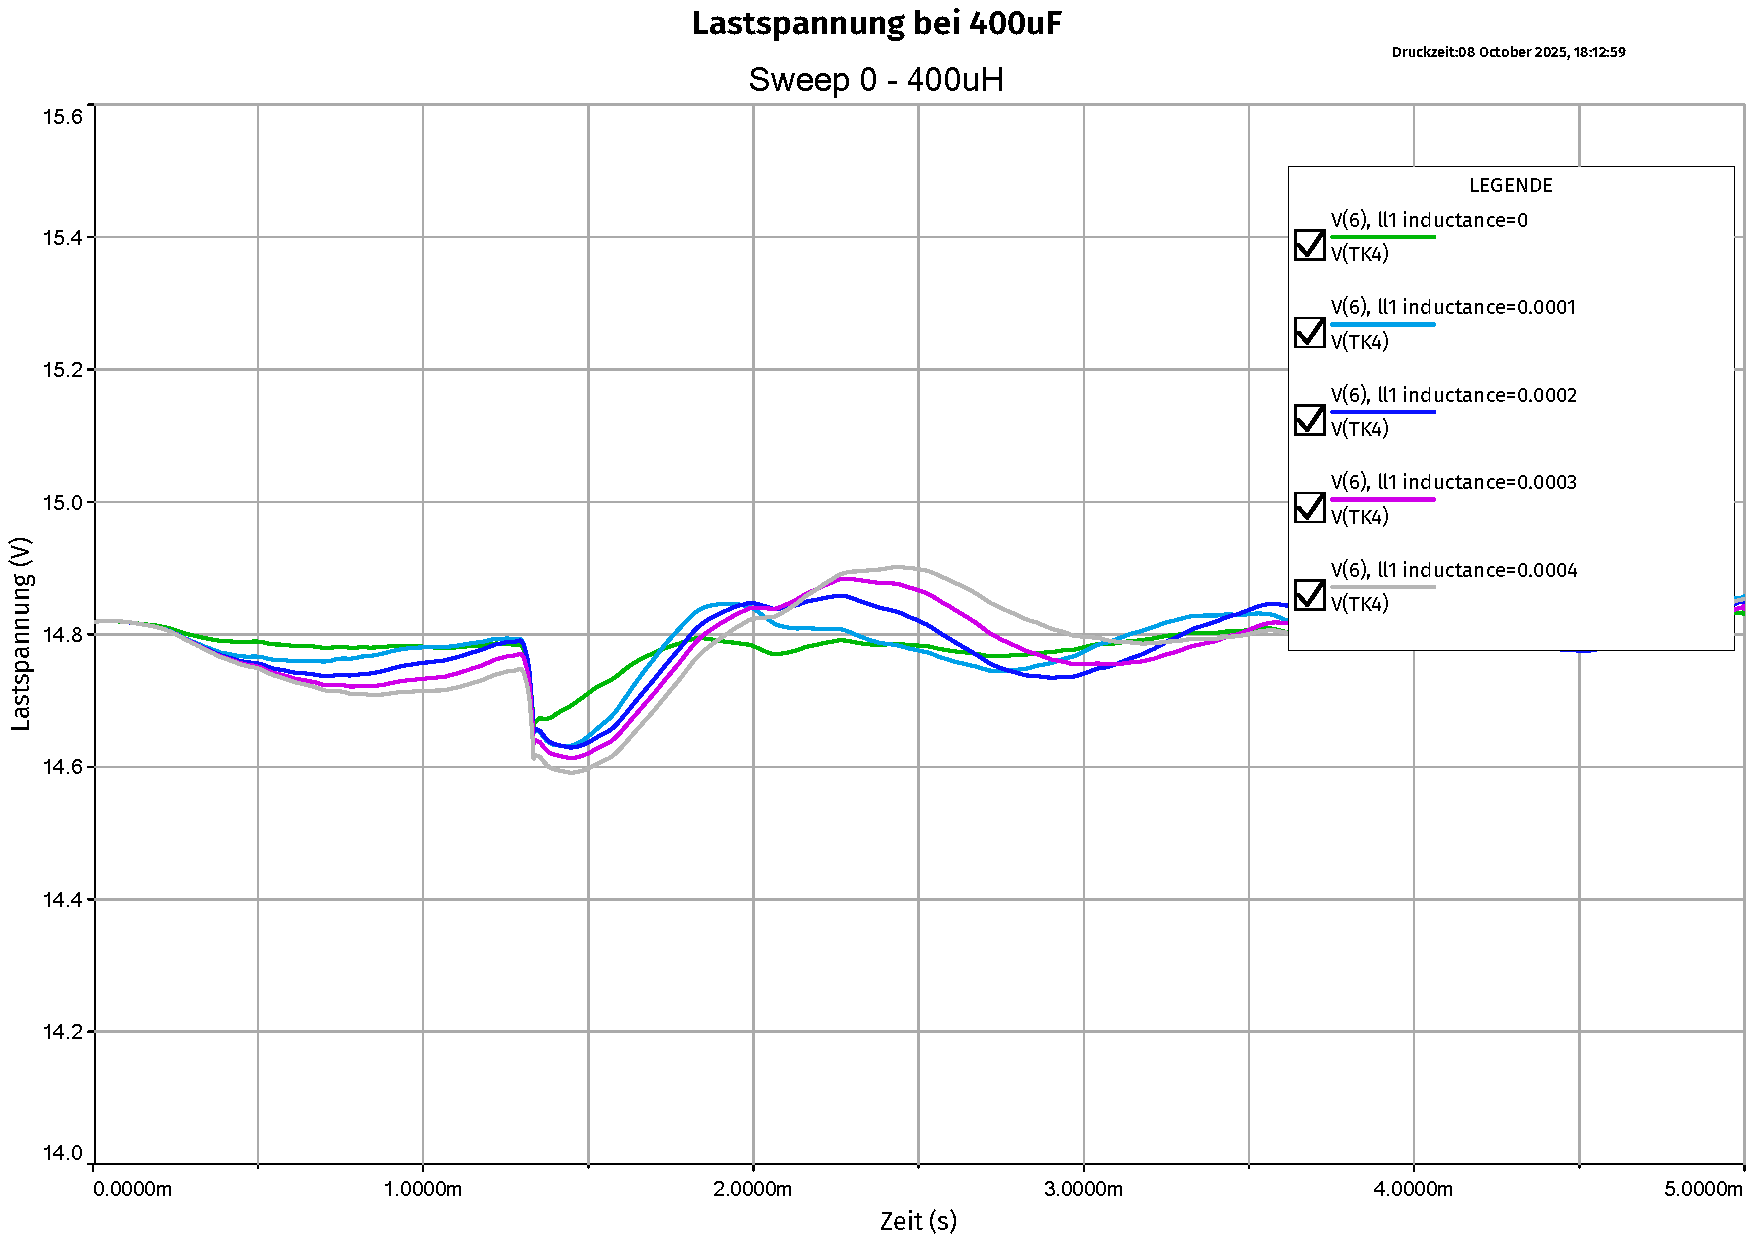
\includegraphics[width=\textwidth]{pictures/2LoadsParallel_Lastspannung bei 400uF_IndSweep0Hto400uH.pdf}
		\caption{Lastspannung bei 400uF und 0-400uH}
		\label{pic:loadvoltage_400uF}
	\end{subfigure}
	\hfill
	\begin{subfigure}{\textwidth*6/13}
		\centering
		\includegraphics[width=\textwidth]{pictures/2LoadsParallel_Speisestrom bei 400uF Kapazität_IndSweep0Hto400uH.pdf}
		\caption{Speisestrom bei 400uF und 0-400uH}
		\label{pic:supplycurrent_400uF}
	\end{subfigure}
	\caption{Lastspannung und Speisestrom bei 400uF und 0-400uH}
	\label{pic:supplycurrent_loadvoltage_400uF}
\end{figure}
So wurde ersichtlich, dass ab ca. 300uF keine deutliche Verbesserung für die Spannungsstabilität mehr erreicht werden kann\footnote{Vergleich von Abbildungen \ref{pic:loadvoltage_300uF} und \ref{pic:loadvoltage_400uF}}. Bei dieser Kapazität ist ab ca. 200uH auch keine Verringerung des Spitzenstromes mehr erkennbar\footnote{Siehe Abbildung \ref{pic:supplycurrent_300uF}}.
Es wurde klar, dass mit einer Kapazität von \textbf{350uF} und \textbf{150uH} der Spannungsbereich auch bei Spitzenströmen zwischen 14.6V und 14.9V un der Speisungsstrom unter 0.9A gehalten werden konnte. Abbildung \ref{pic:simulation_150uH_350uF} zeigt das Verhalten bei einer Lasttransiente mit diesen Bauteilwerten.\\
\begin{figure}[H]
	\centering
	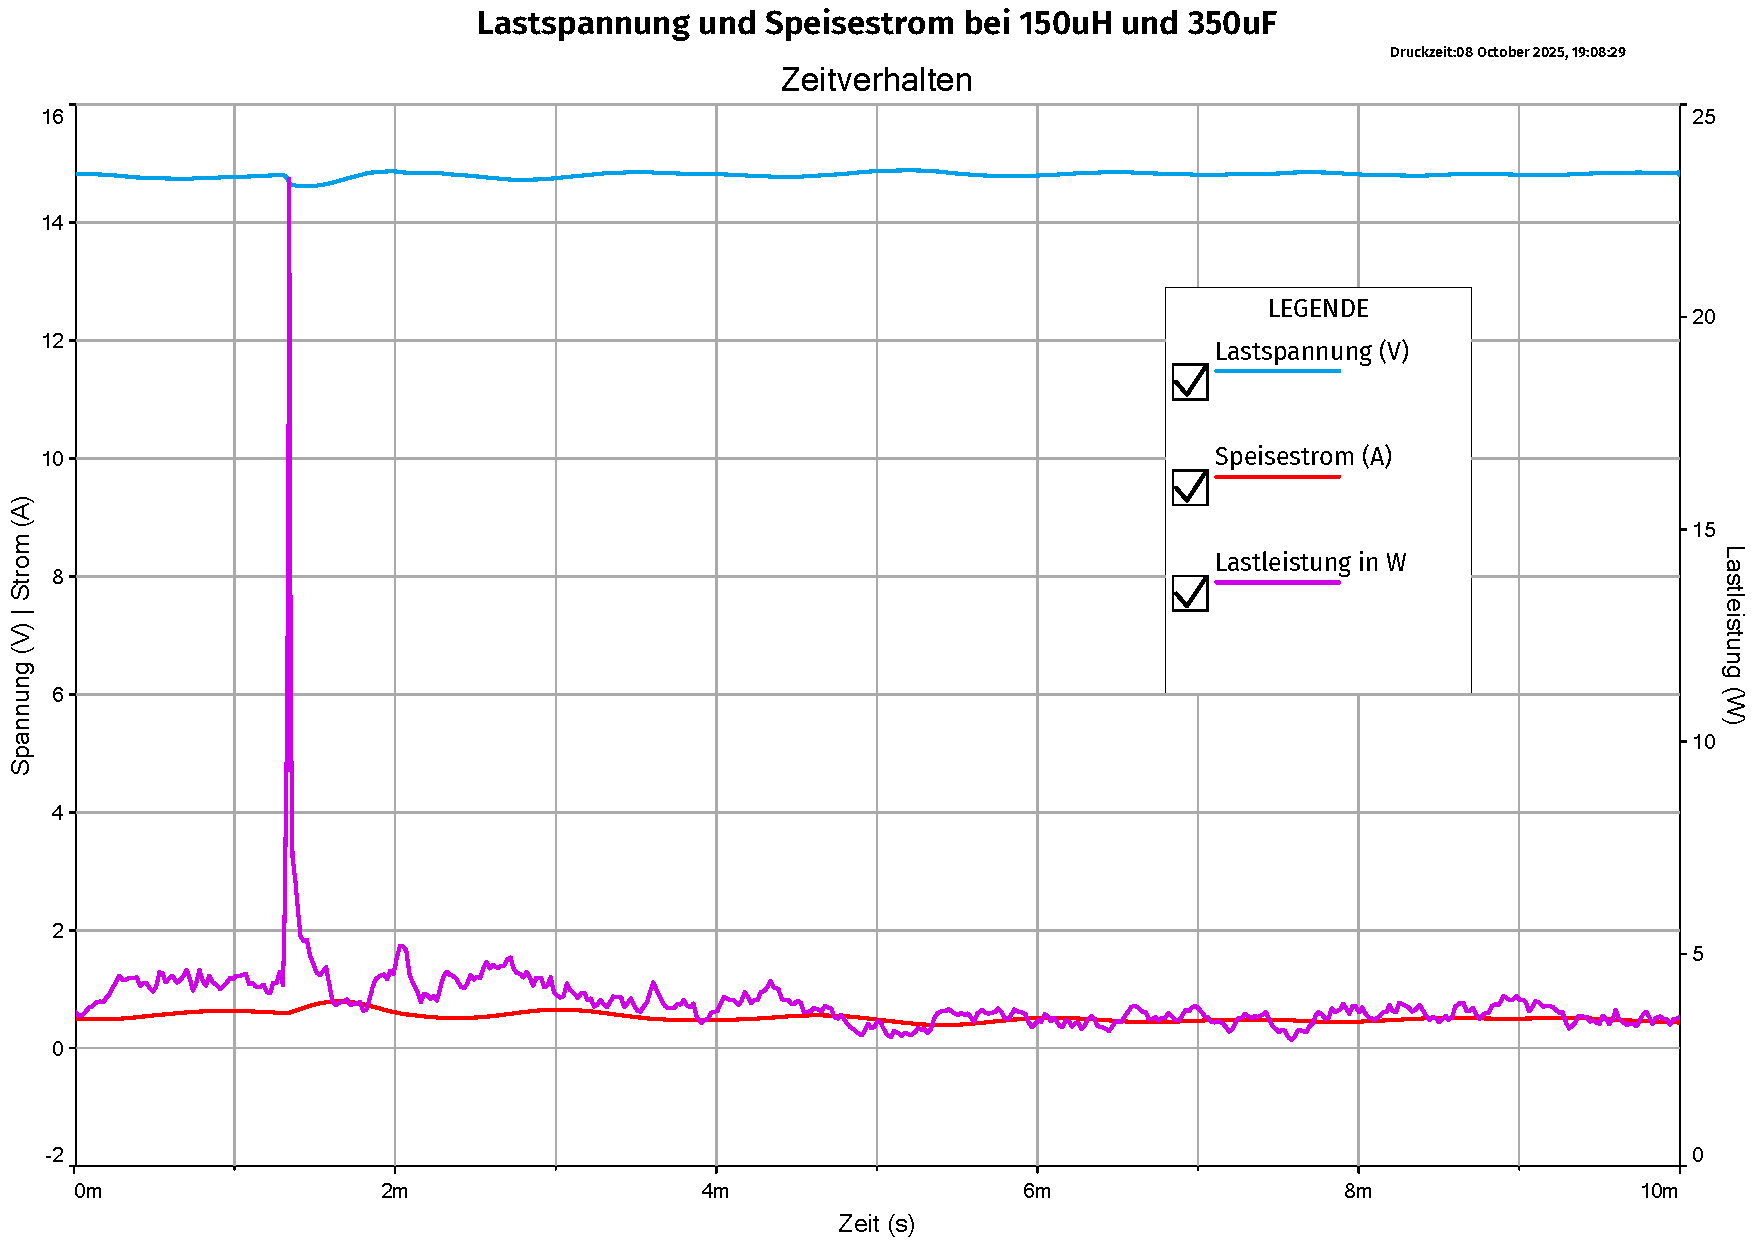
\includegraphics[width=\textwidth*6/8]{pictures/2LoadsParallel_Lastspannung und Speisestrom bei 150uH und 350uF.pdf}
	\caption{Speisungsverhalten bei 150uH und 350uF}
	\label{pic:simulation_150uH_350uF}
\end{figure}
\paragraph{Kapazität}Das Datenblatt des TAS5720 gibt einige Empfehlungen, wie die Kapazität gestalltet werden sollte. Es wird zudem empfohlen, an beiden PVDD-Eingängen einen Kondensator zu platzieren.

\begin{quotation}
	\textit{\textbf{8.2.2.4}
	Select the bulk capacitors at the PVDD inputs for proper voltage margin and adequate capacitance to support the
	power requirements. The TAS5720L/M has very good PVDD PSRR, so the capacitor is more about limiting the
	ripple and droop for the rest of system than preserving good audio performance. The amount of bulk decoupling
	can be reduced as long as the droop and ripple is acceptable. One capacitor should be placed near the PVDD
	inputs at each side of the device. PVDD capacitors should be a low ESR type because they are being used in a
	high-speed switching application.\\
	\textbf{8.2.2.5 }
	Select Decoupling Capacitors
	Good quality decoupling capacitors should be added at each of the PVDD inputs to provide good reliability, good
	audio performance, and to meet regulatory requirements. X5R or better ratings should be used in this
	application. Consider temperature, ripple current, and voltage overshoots when selecting decoupling capacitors.
	Also, the decoupling capacitors should be located near the PVDD and GND connections to the device to
	minimize series inductances.}\\-Quelle: \cite{TAS5720L/M_datasheet}
\end{quotation}
Somit mussten also pro Eingang ein grösserer Kondensator sowie ein kleinerer, etwa 100nF, vorgesehen werden. Da zwei Kanäle zusammen gefiltert werden sollen, sind also insgesamt vier grössere Kondensatoren vorgesehen. Für den grossen Kondensator kamen wegen der DC-Spannung von 15V und den Dimensionen nur Aluminium-Polymer Kondensatoren in Frage. Das Datenblatt gab hier pro Kondensator eine Kapazität von mindestens 100uF an. Hier musste auch der Spitzen-Rippelstrom überprüft werden: Die Simulation gab dabei einen Spitzenstrom von ca. 0.6A pro Kondensator an. Die Hersteller geben jeweils den maximalen Welligkeitsstrom bei Niederfrequenz, 120 Hz, und Hochfrequenz, 100k Hz, an. Die im Testsignal vorkommende Transientendauer von 160us entspräche also 6kHz, oder 3kHz wenn sie als eine Halbwelle interpretiert wird. Welcher Spitzenstrom kann also als Kennwert verwendet werden? Da dies wahrscheinlich nicht so einfach linear interpoliert werden kann, wurde sicherheitshalber der \href{https://www.digikey.ch/de/products/detail/kemet/A782MS107M1JLAS030/21544807}{A782MS107M1JLAS030} gewählt, welcher eine Spannungsfestigkeit von 63V hat und bei 120Hz 800mA aushält. Dimensionen: 10,80mm x 10,30mm x 12,70mm.
\paragraph{Induktivität}Die Spule musste lediglich den neuen Spitzenstrom aushalten und möglichst klein sein. Die Spule \href{https://www.digikey.ch/de/products/detail/w%
	C3%BCrth-elektronik/74404086151/8134307}{74404086151 von Würth Elektronik} erfüllte diese Anforderungen, hatte jedoch mit 355mOhm einen höheren ESR als in der Simulation. Nach einer erneuten Simulation mit diesem ESR-Wert zeigten sich jedoch keine Probleme dadurch. Dimensionen: 8,00mm x 8,00mm x 6,50mm.
\paragraph{Alle 6 Kanäle zusammen entkoppeln?}Es wäre nun möglich gewesen, einen Schritt weiter zu gehen und gleich alle sechs Kanäle mit nur diesen zwei Bauteilen zu entkoppeln. Dies führte jedoch zu einem Spannungseinbruch auf 13.5V und einem Kondensatorstrom von über \textbf{7.1A}, was nicht akzeptabel war.
\subsubsection{Simulation 3x2 Kanäle und 15V-Kennwerte}Nun wurde die Last mit den Entkoppelungselementen zwei mal kopiert, so dass der Parallelbetrieb von allen sechs Kanälen simuliert werden konnte. Dabei blieb die Lastspannung zwischen \textbf{14.2V und 14.4V} und der Spitzen-Speisungsstrom bei max. \textbf{2.11A}.\\
\begin{center}
	\begin{minipage}{\textwidth*7/8}
		\centering
		{\large Aus diesen Ergebnissen wurde entschieden, jeweils zwei Kanäle mit insgesamt vier \textbf{100uF Aluminium-Polymer Kondensatoren} und einer \textbf{150uH Drosselspule} zu entkoppeln.}
	\end{minipage}
\end{center}
\subsection{Schaltregler}
Mit den nun bekannten Kennwerten zum Spitzenstrom wurde versucht, die Speisung mit einem einzelnen Schaltregler, ohne LDO, zu regeln. Auch hier wurde ChatGPT eingesetzt, um eine Empfohlene Bauteilliste zu generieren, jedoch schlug die KI hier fast ausschliesslich uModules\footnote{Schaltregler mit integrierten Passivelementen, meist die Ausgangsspule.} mit Ausgangsströmen von 6-8A vor oder mit einer maximalen Ausgangsspannung von 15V. Hier zeigte sich, dass viele Datenblätter die Angaben nur bis 12V machten. Diese Speisespannung hätte allerdings Nachteile für die Endstufe gebracht.\\Als weitere Beobachtung schien die KI fast ausschliesslich Produkte von Texas Instruments oder Analog Devices vorzuschlagen. Als weiterer Hersteller kam \href{https://www.monolithicpower.com/en/}{MPS} infrage, deren einziges Modul welches die Anforderung erfüllt (\href{https://www.monolithicpower.com/en/documentview/productdocument/index/version/2/document_type/Datasheet/lang/en/sku/MPM3530GRF/}{MPM3530}) ist 15V jedoch wieder die maximale Ausgangsspannung.\\Letztendlich wurde folgender Promt eingesetzt, da auch eine 5V-Spannung erzeugt werden musste:
\begin{center}
	\vspace{3mm}
	\begin{parbox}[][][]{\textwidth*3/4}
		{\textit{\dotfill\\recommend me some switching regulator ICs which can handle an input voltage of 24V, dual output voltage of 15V and 5V, peak Current of 2.2A. Fokus on low noise, high PSRR. limiter}\\.\dotfill.}
	\end{parbox}
\end{center}\vspace{3mm}
Die zusammengefasste Antwort darauf:
\\.\dotfill.\\\textit{
\begin{itemize}
	\item \textbf{Top Pick}: Analog Devices — LT8650S (Silent-Switcher®2, dual channel)
	\item Analog Devices — LT8648S
	\item 2x Analog Devices — LTM4613 µModule
	\item 2x Texas Instruments — TPSM33625 (power module, 3–36 V VIN, 2.5 A)
\end{itemize}}
.\dotfill.\\
\paragraph{Kurzevaluation}Der LT8648S ist mit einem einzelnen Ausgang und einem Nennstrom von 15A viel zu gross dimensioniert. Zweimal ein uModule zu nutzen vernichtet die Vorteile dieses Ansatzes. Als Alternative zum Top Pick LT8650S wurde zusätzlich zu dieser Liste manuell der TI TPSM64406, ein Dual Output uModule, gesucht und ins Auge gefasst. Tabelle \ref{tab:Vergleich_LT8650S_TPSM64406} zeigt den Direktvergleich zwischen den Modellen. Es gibt viele Ähnlichkeiten und von der Performance her sind beide auf dem selben Level. Der Vergleich zwischen den Transientenverhalten (Abb. \ref{pic:transient_behv}) zeigte jedoch durch die externe Kompensation ein leicht besseres Verhalten. Jedoch waren bei diesem Chip die Kosten leicht höher und brauchte leicht mehr Platz auf dem PCB.
\subsubsection{Direktvergleich von LT8650S und TPSM64406}
\begin{table}[H]
	\centering
	\setstretch{1.5}
	\begin{tabularx}{\textwidth*7/8}{>{\hsize=.8\hsize}XXX}
		&{\large \textbf{LT8650S}} & {\large \textbf{TPSM64406}}\\\toprule
		\textbf{Hersteller}&Analog Devices&Texas Instruments\\\midrule
		\textbf{Typ}&Synchronous Step-Down Silent Switcher 2&High-density, dual 3A output power module\\\midrule
		\textbf{Induktivität}&extern&integriert\\\midrule
		\textbf{Kapazität}&extern&extern\\\midrule
		\textbf{Baugrösse}&4mm x 6mm x 0.94mm&7mm x 6.5mm x 2mm\\\midrule
		\textbf{geschätzte Grösse des recomm. Layout}&\textit{ca.} 20mm x 20mm&\textit{ca.} 10mm x 20mm\\\midrule
		\textbf{Ausgangsspannungen}&Keine Direkte Angabe&0.8-16V\\\midrule
		\textbf{Schaltfrequenz}&300kHz to 3MHz& 300kHz to 2200kHz\\\midrule
		\textbf{max. Ausgangsstrom\newline{\small Ein Kanal}}&3A&4A\\\midrule
		\textbf{Output Ripple}&<10mVP-P\newline{\small Hängt auch von externen Komponenten ab}&1\%\newline{\small Output voltage regulation des Design 1}\\\midrule
		\textbf{Features}&\textendash Optional Spread Spectrum Modulation\newline\textendash Burst Mode® Operation\newline\textendash  Optional External VC Pin: Fast Transient Response\newline\textendash Forced Continuous Mode\newline\textendash programmable Soft-Start&\textendash Negative output voltage capability\newline\textendash External bias option\newline\textendash dual input paths\newline\textendash integrated capacitors\newline\textendash Precision enable input\newline\textendash internal Soft-Start\\\midrule
		\textbf{Stückpreis auf DigiKey}&12.69 CHF&11.10 CHF\\\bottomrule
	\end{tabularx}
	\caption{Direktvergleich zwischen zwei Schaltreglern}
	\label{tab:Vergleich_LT8650S_TPSM64406}
\end{table}
\paragraph{Fazit}Hier war die Entscheidung recht schwierig. Die Vor- und Nachteile heben sich jeweils sehr gut auf. Auch die Effizienz war bei beiden Modellen mit den gegebenen Spannungen und Strömen bei ca. 92\%. Jedoch wurde der LT8650S als einfacher zu integrieren\footnote{Das Landing Pattern des TPSM64406 ist recht komplex.} erachtet und hatte leicht besseres Verhalten bei Lasttransienten.
\begin{center}
	\begin{minipage}{\textwidth*7/8}
		\centering
		{\large Daher wurde der LT8650S als Schaltregler ausgewählt.}
	\end{minipage}
\end{center}
\begin{figure}[H]
	\centering
	\begin{subfigure}{\textwidth*6/8}
		\centering
		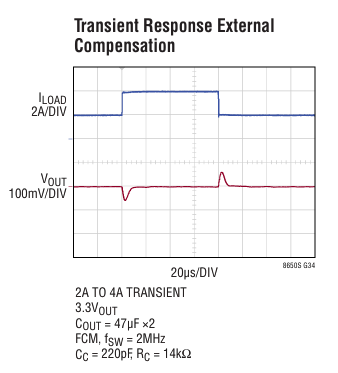
\includegraphics[width=\textwidth*1/2]{pictures/LT8650S_transient_behv.png}
		\caption{Transientenverhalten des LT8650S, ca. 50mV-Ausschläge}
		\label{pic:transient_behv_LT8650S}
	\end{subfigure}
	\vspace{5mm}
	\begin{subfigure}{\textwidth*6/8}
		\centering
		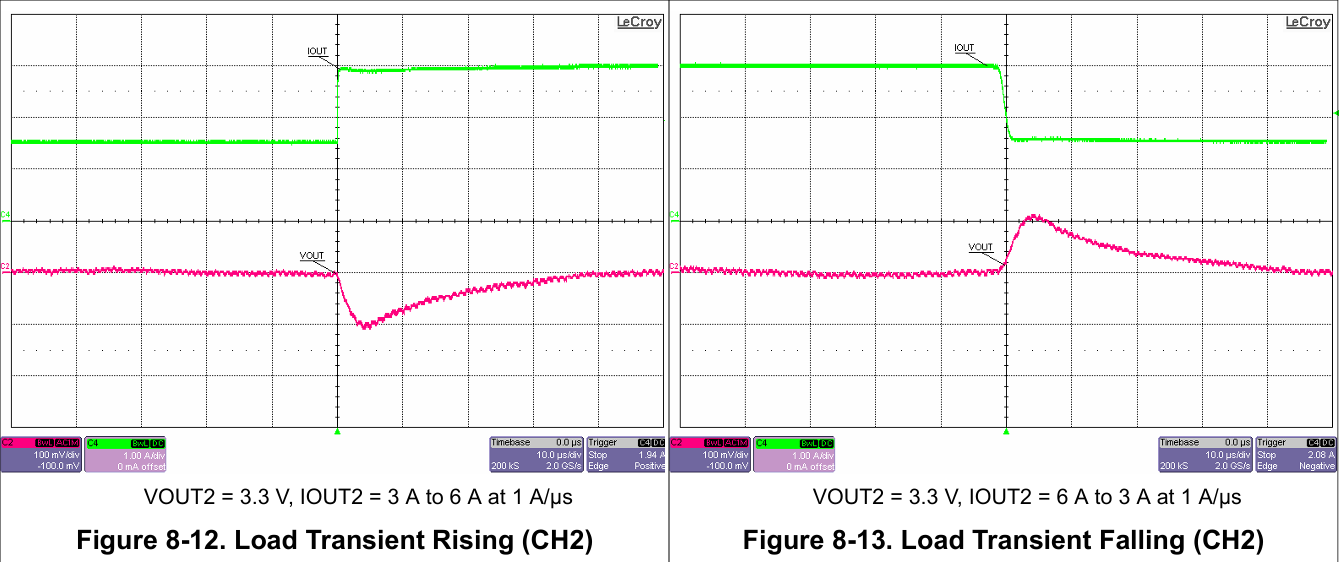
\includegraphics[width=\textwidth]{pictures/TPSM64406_transient_behv.png}
		\caption{Transientenverhalten des TPSM64406, ca. 100mV-Ausschläge}
		\label{pic:transient_behv_TPSM64406}
	\end{subfigure}
	\caption{Der Vergleich des Transientenverhalten zeigte einen leichten Unterschied.}
	\label{pic:transient_behv}
\end{figure}